\documentclass[11pt]{amsart}

\usepackage[dutch]{babel}
\usepackage{a4wide}
\usepackage{graphicx}
%\setlength{\parindent}{0pt}

\newtheorem*{vraag}{Vraag}
\theoremstyle{definition}
\newtheorem*{uitwerking}{Uitwerking}
\newtheorem*{matlab}{Matlab-code}

\newcommand{\R}{\mathbb{R}}
\newcommand{\N}{\mathbb{N}}
\newcommand{\Z}{\mathbb{Z}}
\newcommand{\C}{\mathbb{C}}
\newcommand{\A}{\mathbb{A}}
\newcommand{\Q}{\mathbb{Q}}
\newcommand{\F}{\mathbb{F}}
\newcommand{\f}{\varphi}
\newcommand{\e}{\varepsilon}
\renewcommand{\d}{\delta}

\begin{document}

\title{Systems \& Control Theory -- Huiswerk serie 1}
\author{Jan Westerdiep, Okke van Garderen}
\maketitle

\section*{Assignment 1}
\begin{uitwerking}
  Als eerste kunnen we uit \texttt{exercise\_08\_1\_1.m} destilleren dat
  \[
  T = \begin{bmatrix} t_1 & t_2 & 0 \\ t_3 & t_4 & 0 \\ 0 & 0 & 1 \end{bmatrix},
  L = \begin{bmatrix} a & 0 & 0 \\ 0 & b & 0 \\ 0 & 0 & 1 \end{bmatrix},
  A = T L T^{-1}, x_0 = \begin{pmatrix} (t_1 + t_2)/3 \\ (t_3 + t_4)/3 \\ 1/3 \end{pmatrix}.
  \]
  Merk gelijk op dat dit een eigendecompositie van $A$ is.

  Dit heeft als gevolg dat de iteratie $x_k = A x_{k-1} = \ldots = A^k x_0$ wordt:
  \[
  x_k = A^k x_0 = (T L T^{-1})^k x_0 = TL^k T^{-1} x_0 = T L^k \begin{pmatrix} 1/3 \\ 1/3 \\ 1/3 \end{pmatrix}.
  \]

  Nu is
  \[
  L^k \begin{pmatrix} 1/3 \\ 1/3 \\ 1/3 \end{pmatrix} = 1/3 L^k \begin{pmatrix} 1 \\ 1 \\ 1 \end{pmatrix} = 1/3 \begin{bmatrix} a^k & 0 & 0 \\ 0 & b^k & 0 \\ 0 & 0 & 1^k \end{bmatrix}\begin{pmatrix} 1 \\ 1 \\ 1 \end{pmatrix} = 1/3 \begin{pmatrix} a^k \\ b^k \\ 1 \end{pmatrix}
  \]
  dus
  \[
  x_k = 1/3 \begin{pmatrix} t_1 a^k + t_2 b^k \\ t_3 a^k + t_4 b^k \\ 1 \end{pmatrix}.
  \]

  Dit wordt ook duidelijk in de plot: de derde co\"ordinaat van $x_k$ is altijd $1/3$.
\end{uitwerking}

\begin{matlab}~

\begin{verbatim}
  function void = ass1
  n1 = 10191429;
  n2 = 18008105;
  Snummer = [n1 ; n2 ];

  exercise_08_1_1

  Y = A;
  X = x0;
  for tel = 1:6,
  X = [X Y*X];
  Y = Y*Y;
  end

  plot3(X(1,:),X(2,:),X(3,:),"+"); grid;
  end
\end{verbatim}
\end{matlab}

\section*{Assignment 2}
\begin{itemize}
\item[Deelvraag 1.]
  \begin{uitwerking}
    Er geldt dat de polen van $f$ worden gegeven door de nulpunten van de 
    noemer en haar nulpunten door de nulpunten van de teller.
    We hoeven dus alleen een kort stukje matlab code te gebruiken om
    deze te vinden en te plotten.
  \end{uitwerking}
  \begin{matlab}~
\begin{verbatim}
n1 = 10191429;
n2 = 18008135;
Snummer = [n1 ; n2]
exercise_08_1_2

polen = roots(noemer)
nulp  = roots(teller)
%plot de functie rond de polen
for i=1:size(polen)(1)
  figure(i);
  x = polen(i);
  xs = [x - 0.1 : 0.001: x+0.1];
  plot(xs,arrayfun(@(x) polyval(teller,x)/polyval(noemer,x),xs));
end
%plot de functie rond de nulpunten
for i=1:size(nulp)(1)
  figure(i);
  x = nulp(i);
  xs = [x - 0.1 : 0.001: x+0.1];
  plot(xs,arrayfun(@(x) polyval(teller,x)/polyval(noemer,x),xs));
end
\end{verbatim}
  \end{matlab}
\item[Deelvraag 2.]
  \begin{uitwerking}
    We merken op dat we een staartdeling uit kunnen voeren van de teller door de noemer, waarbij we doorgaan tot de 6e negatieve macht van $x$. Hiervoor hebben we het volgende algoritme geschreven dat de staartdeling uitvoert voor 2 willekeurige polynomen.
    \end{uitwerking}
\begin{matlab}
\begin{verbatim}
function [a,z,q] = divide_polys(p,q,d)
  % IN: p,q -> polynoom coeffs van polys in p/q, d minimale graad
  % UIT: a -> lijst van coefs, z,q -> coefs van polys zodat z/q = R
  lp = size(p);
  p = [p zeros(1,d)];
  1 = [q zeros(1,d)];
  a = zeros(1,d);

  s = 1;
  while p(s) == 0
        s=s+1 ;
  end

  for i=1:d
    a(i) = p(i)/q(s);
    for j=i:lp+d
      p(j) = p(j) - a(i) * q(j-i+1);
    end
  end
  z = p
end
\end{verbatim}
\end{matlab}
\item[Deelvraag 3.]
  Onze functie $f(x) =\frac{t(x)}{n(x)}$ heeft een pool in het punt $0$,
  dit betekent dat $\lim_{x\to 0} |f(x)| = \infty$. Stel dat we $f$ kunnen schrijven als:
  \[
  f(x) = b_0 + b_1 x + \ldots + b_n x^n + x^n S_n(x),
  \]
  met $S_n$ een rationele functie, dan impliceert dit dat $S_n$ ook een pool
  moet hebben in het punt $0$ en dit is niet wat we willen.

\end{itemize}
\section*{Assignment 3}
\begin{uitwerking}
  Onze matrix $A_r$ is een random $6 \times 3$ matrix maal een random $3 \times 6$ matrix. We verwachten dus dat $A_r$ maximaal\footnote{Omdat we met random waarden werken, kan $A_r$ natuurlijk ook bijvoorbeeld singulier zijn. Dat is in ons geval niet zo.} rang 3 heeft. Wanneer we de matrix $A$ maken zoals voorgeschreven, en daarop de singuliere waarden-decompositie vinden, blijkt zij echter van volle rang te zijn (hoewel, met drie zeer kleine singuliere waarden).

  Laat $U, S, V = svd(A)$. Dan weten we dat $A = U S V^T$. De voor de hand liggende matrix $A_n$ wordt nu $A_n := U S' V^T$ met $S'$ d\'ie matrix met singuliere waarden kleiner dan onze nauwkeurigheid ($= 1/1000$) gelijk nul gesteld. Dan
  \[
  \Delta A := A - A_n = U S V^T - U S' V^T = U(S - S')V^T = U \Delta S V^T,
  \]
  met $\Delta S$ een matrix waar enkel nullen staan, samen met $\e_4, \e_5, \e_6$ op de onderste plekken van de diagonaal. Een cel $(\Delta A)_{ij}$ wordt zo
  \[
  (\Delta A)_{ij} = (U \Delta S)_{i,:} \cdot V_{:,j} = u_4 v_4 \e_4 + u_5 v_5 \e_5 + u_6 v_6 \e_6
  \]
  het inproduct van twee vectoren. Hierbij is $u_k$ de $k$-de co\"oordinaat van de rijvector $U_{i,:}$ en $v_k$ de $k$-de co\"oordinaat van de (kolom)vector $V_{:,j}$.

  Omdat $U$ en $V$ unitair zijn, en door $\|x \|_1 \leq \sqrt{n} \|x\|_2$, geldt $\sum w_k \leq \sqrt{6}$ voor $w \in \{u, v\}$. Neem het worst case: $w_k = \sqrt{6}/3$ voor $w \in \{u, v\}, k \in \{4, 5, 6\}$. Dan staat er
  \[
  (\Delta A)_{i,j} = 3 \cdot (\sqrt{6}/3)^2 \cdot (\e_4 + \e_5 + \e_6) = 2 (\e_4 + \e_5 + \e_6) < 2 \cdot 3 \cdot 1/1000 = 6/1000.
  \]

  We hebben helaas in een \emph{worst worst case} geval niet een verschil van kleiner dan $1/1000$ kunnen halen,\footnote{Gebruikmakend van de stelling die in de uitwerking van assignment 4 gegeven wordt, is het simpel aan te tonen dat hoewel $A_n$ misschien niet het verschil minimaliseert in de $1$-norm, maar wel in de $2$-norm.} maar $6/1000$ is ook prima. Overigens is het verschil in onze specifieke matrix gewoon $0.37/1000$, prima binnen de marge.
\end{uitwerking}
\begin{matlab}~

\begin{verbatim}

  n1 = 10191429;
  n2 = 18008105;
  Snummer = [n1 ; n2 ];
  randn('state', Snummer);

  Areal = randn(6,3) * randn(3,6);
  A = round(1000*Areal)/1000;

  [U, S, V] = svd(A)
  for i = 1:6,
  if S(i,i) < 1/1000
  S(i,i) = 0;
  end
  end
  S
  Anew = U*S*V';
  max(abs((Anew - A)(:))) %< 6/1000
\end{verbatim}
\end{matlab}

\section*{Assignment 4}
\begin{uitwerking}
  Voor deze opgave zullen we het boek \emph{Numerical Linear Algebra} van Trefethen en Bau gebruiken.

  Kijk namelijk naar stelling 5.8:
  \begin{quote}
    Let $A = U \Sigma V^*$. For any $\nu$ with $0 \leq \nu \leq r$, where $r = rk(A)$, define
    \[
    A_\nu = \sum_{j=1}^\nu \sigma_j u_j v_j^*;
    \]
    if $\nu = p = \min{\{m,n\}}$, define $\sigma_{\nu + 1} = 0$. Then
    \[
    \| A - A_\nu \|_2 = \inf_{B \in \C^{m \times n}, rank(B) \leq \nu} \| A - B \|_2 = \sigma_{\nu + 1}.
    \]
  \end{quote}
  In andere woorden: de matrix met rang $\nu$ die het dichtste bij $A$ komt van alle matrices met rank $\nu$, kunnen we gewoon vinden! De toepassing hiervan komt uit opgave 9.3:

  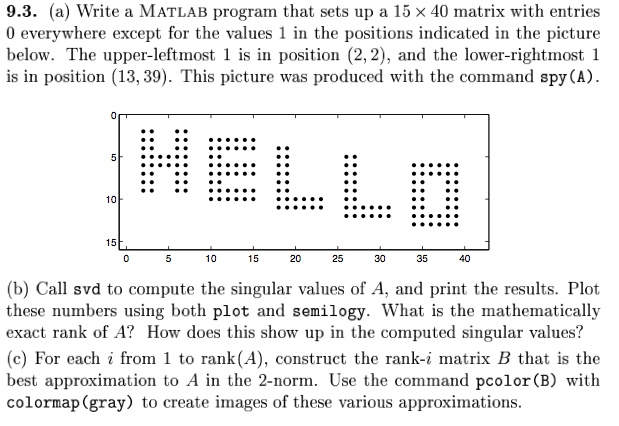
\includegraphics[width=\textwidth]{bla.png}

  Het resultaat uit opgave 9.3c is nu zeer mooi om te zien:

  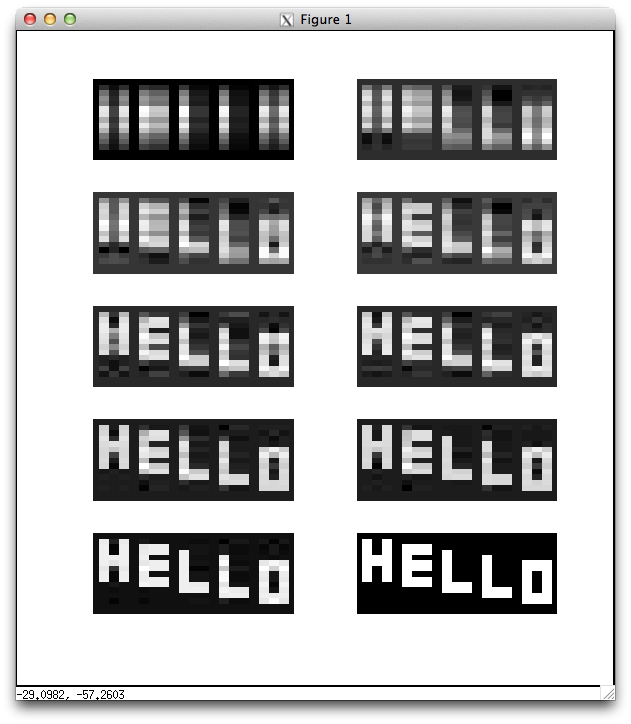
\includegraphics[width=\textwidth]{opg9_3c.png}

\end{uitwerking}
\begin{matlab}~
\begin{verbatim}
  A = [
    0 0 0 0 0 0 0 0 0 0 0 0 0 0 0 0 0 0 0 0 0 0 0 0 0 0 0 0 0 0 0 0 0 0 0 0 0 0 0 0;
    0 1 1 0 0 1 1 0 0 0 0 0 0 0 0 0 0 0 0 0 0 0 0 0 0 0 0 0 0 0 0 0 0 0 0 0 0 0 0 0;
    0 1 1 0 0 1 1 0 0 1 1 1 1 1 1 0 0 0 0 0 0 0 0 0 0 0 0 0 0 0 0 0 0 0 0 0 0 0 0 0;
    0 1 1 0 0 1 1 0 0 1 1 1 1 1 1 0 0 1 1 0 0 0 0 0 0 0 0 0 0 0 0 0 0 0 0 0 0 0 0 0;
    0 1 1 1 1 1 1 0 0 1 1 0 0 0 0 0 0 1 1 0 0 0 0 0 0 1 1 0 0 0 0 0 0 0 0 0 0 0 0 0;
    0 1 1 1 1 1 1 0 0 1 1 1 1 1 1 0 0 1 1 0 0 0 0 0 0 1 1 0 0 0 0 0 0 1 1 1 1 1 1 0;
    0 1 1 0 0 1 1 0 0 1 1 1 1 1 1 0 0 1 1 0 0 0 0 0 0 1 1 0 0 0 0 0 0 1 1 1 1 1 1 0;
    0 1 1 0 0 1 1 0 0 1 1 0 0 0 0 0 0 1 1 0 0 0 0 0 0 1 1 0 0 0 0 0 0 1 1 0 0 1 1 0;
    0 1 1 0 0 1 1 0 0 1 1 1 1 1 1 0 0 1 1 0 0 0 0 0 0 1 1 0 0 0 0 0 0 1 1 0 0 1 1 0;
    0 0 0 0 0 0 0 0 0 1 1 1 1 1 1 0 0 1 1 1 1 1 1 0 0 1 1 0 0 0 0 0 0 1 1 0 0 1 1 0;
    0 0 0 0 0 0 0 0 0 0 0 0 0 0 0 0 0 1 1 1 1 1 1 0 0 1 1 1 1 1 1 0 0 1 1 0 0 1 1 0;
    0 0 0 0 0 0 0 0 0 0 0 0 0 0 0 0 0 0 0 0 0 0 0 0 0 1 1 1 1 1 1 0 0 1 1 1 1 1 1 0;
    0 0 0 0 0 0 0 0 0 0 0 0 0 0 0 0 0 0 0 0 0 0 0 0 0 0 0 0 0 0 0 0 0 1 1 1 1 1 1 0;
    0 0 0 0 0 0 0 0 0 0 0 0 0 0 0 0 0 0 0 0 0 0 0 0 0 0 0 0 0 0 0 0 0 0 0 0 0 0 0 0;
    0 0 0 0 0 0 0 0 0 0 0 0 0 0 0 0 0 0 0 0 0 0 0 0 0 0 0 0 0 0 0 0 0 0 0 0 0 0 0 0
  ];

  [U S V] = svd(A);
  %A heeft 10 singuliere waarden boven nul en is dus van rang 10 (stelling 5.1)
  for i = 1:10,
  Av = zeros(size(A));
  for j = 1:i, %zie stelling 5.8
  Av = Av + S(j,j) * U(:,j) * V(:,j)';
  end
  subplot(5,2,i)
  imagesc(Av)
  axis("off")
  colormap(gray)
  end
\end{verbatim}
\end{matlab}

\end{document}
